\documentclass[11pt]{article}

\usepackage{amsmath}
\usepackage{amsthm}
\usepackage{amssymb}
\usepackage[pdftex]{graphicx}
\usepackage{subfig}
\usepackage{wrapfig}
\usepackage{enumerate}
\usepackage{fancyhdr}
\usepackage{listings}
\usepackage{textcomp}
\usepackage[
  pdftitle={},%
  pdfauthor={},%
  pdfsubject={},%
  pdfkeywords={},%
  pdfstartview=FitH,%
  bookmarks=true,%
  bookmarksopen=true,%
  breaklinks=true,%
  colorlinks=true,%
  linkcolor=red,anchorcolor=black,%
  citecolor=green,filecolor=cyan,%
  menucolor=red,urlcolor=magenta,%
  pdftex]{hyperref}
\usepackage{makeidx}
\usepackage{subfig}
\usepackage{wrapfig}
\usepackage[usenames]{color}
\usepackage[sectionbib]{chapterbib}
\usepackage[square,numbers,sort&compress,sectionbib,nonamebreak]{natbib}
\usepackage[margin=1.3in,letterpaper,portrait]{geometry}
\usepackage[Bjarne]{fncychap}
\usepackage{minitoc} 
\usepackage{float}
\usepackage{tikz}
\makeindex

\renewcommand\familydefault{\sfdefault}

%\usepackage{../../styles/clrscode3e}
%\usepackage{../../styles/clrmac}
%\usepackage{../../styles/supertech-sig}

%%%%%%%%%% Start TeXmacs macros
% macro for todo entries
%The first argument is the name of the person who should do the specified tak. This argument is optional and defaults to ``scribe''. 
%The second argument describes the type of the task. Tasks can be 
%missing 
%expand 
%clarify 
%reference 
%incorrect 
%editing 

%The third argument contains the message describing what needs to be done. 
\definecolor{CornSilk}{rgb}{1,1,.88}
\newcommand{\todo}[3][scribe]{\textbf{\textcolor{red}{TODO: #2}} \textit{\textcolor{green}{@#1}\textcolor{blue}{ : #3}}}
%aside note: 
\newcommand{\sidenote}[1]{\fcolorbox{black}{CornSilk}{\parbox{6 in}{\textit{\textbf{\Large{Did You Know?}}}\newline #1}}}
\newcommand{\nbdiscussion}[1]{\footnote{\fcolorbox{black}{CornSilk}{\parbox{6 in}{\textit{\textbf{\Large{NB Discussion}}}\newline #1}}}}
\newcommand{\faq}[2]{\fcolorbox{black}{CornSilk}{\parbox{6 in}{\textbf{\textit{\Large{FAQ}}}\newline 
\begin{description} 
\item[\textbf{Q:}] #1
\newline 
\item[\textbf{A:}] #2
\end{description} }}}
\newcommand{\hilight}[1]{\colorbox{yellow}{#1}}
\newcommand{\tmabbr}[1]{#1}
\newcommand{\tmem}[1]{{\em #1\/}}
\newcommand{\tmop}[1]{\ensuremath{\operatorname{#1}}}
\newcommand{\tmstrong}[1]{\textbf{#1}}
\newcommand{\tmtextit}[1]{{\itshape{#1}}}
\newcommand{\tmtexttt}[1]{{\ttfamily{#1}}}
\newcommand{\getdir}{images}
\newcommand{\keyword}[1]{\index{#1|textbf}}
\newcommand{\mainword}[1]{\textbf{#1}}
\newenvironment{enumeratenumeric}{\begin{enumerate}[1.] }{\end{enumerate}}
\newenvironment{itemizedot}{\begin{itemize} \renewcommand{\labelitemi}{$\bullet$}\renewcommand{\labelitemii}{$\bullet$}\renewcommand{\labelitemiii}{$\bullet$}\renewcommand{\labelitemiv}{$\bullet$}}{\end{itemize}}
\newenvironment{tmparsep}[1]{\begingroup\setlength{\parskip}{#1}}{\endgroup}

 %%%%%%%%%% End TeXmacs macros

%set the margins to a reasonable value 
%\addtolength{\oddsidemargin}{-.75in}
%\addtolength{\evensidemargin}{-.75in}
%\addtolength{\textwidth}{1.5in}
%\addtolength{\topmargin}{-.875in}
%\addtolength{\textheight}{1.75in}

\usepackage{calc}

\makeatletter
\newcommand{\DESCRIPTION@original@item}{}
\let\DESCRIPTION@original@item\item
\newcommand*{\DESCRIPTION@envir}{DESCRIPTION}
\newlength{\DESCRIPTION@totalleftmargin}
\newlength{\DESCRIPTION@linewidth}
\newcommand{\DESCRIPTION@makelabel}[1]{\llap{#1}}%
\newcommand{\DESCRIPTION@item}[1][]{%
  \setlength{\@totalleftmargin}%
       {\DESCRIPTION@totalleftmargin+\widthof{\textbf{#1 }}-\leftmargin}%
  \setlength{\linewidth}
       {\DESCRIPTION@linewidth-\widthof{\textbf{#1 }}+\leftmargin}%
  \par\parshape \@ne \@totalleftmargin \linewidth
  \DESCRIPTION@original@item[\textbf{#1}]%
}
\newenvironment{DESCRIPTION}
  {\list{}{\setlength{\labelwidth}{0cm}%
           \let\makelabel\DESCRIPTION@makelabel}%
   \setlength{\DESCRIPTION@totalleftmargin}{\@totalleftmargin}%
   \setlength{\DESCRIPTION@linewidth}{\linewidth}%
   \renewcommand{\item}{\ifx\@currenvir\DESCRIPTION@envir
                           \expandafter\DESCRIPTION@item
                        \else
                           \expandafter\DESCRIPTION@original@item
                        \fi}}
  {\endlist}
\makeatother

% Macros for proofs, theorems, etc.
\theoremstyle{plain}% default
\newtheorem{thm}{Theorem}[section]
\newtheorem{lem}[thm]{Lemma}
\newtheorem{prop}[thm]{Proposition}
\newtheorem*{cor}{Corollary}
\newtheorem*{KL}{Klein’s Lemma}
\theoremstyle{definition}
\newtheorem{defn}{Definition}[section]
\newtheorem{conj}{Conjecture}[section]
\newtheorem{exmp}{Example}[section]
\theoremstyle{remark}
\newtheorem*{rem}{Remark}
\newtheorem*{note}{Note}
\newtheorem{case}{Case}

\newenvironment{definition}[1][Definition]{\begin{trivlist}
\item[\hskip \labelsep {\bfseries #1}]}{\end{trivlist}}
\newenvironment{example}[1][Example]{\begin{trivlist}
\item[\hskip \labelsep {\bfseries #1}]}{\end{trivlist}}
\newenvironment{remark}[1][Remark]{\begin{trivlist}
\item[\hskip \labelsep {\bfseries #1}]}{\end{trivlist}}



\begin{document}

\title{{\small 6.830 Term Project - Spring 2013}\\Machine Learning Algorithms for In-Database Analytics}
\author{Franck Dernoncourt \& Sumaiya Nazeen}
\maketitle 

\abstract{Our project focused on extending the functionality of MADlib. MADlib is an open source machine learning and statistics library which works with Postgres or Greenplum to provide in-database analytics. Although some machine learning algorithms have been implemented in MADlib, there is room for additional contributions. We implemented two different machine learning algorithms, symbolic regression with genetic programming and adaptive boosting for MADlib, and are in the process of contributing our code to the MADlib community codebase. We also assess the performance of our implementations and compare their performance with the same algorithms outside MADlib.}

\section{Introduction}
\label{sect:introduction}
Traditionally, large databases were mainly used for {\itshape data warehousing} i.e. accounting purposes in enterprises, supporting financial record-keeping and reporting at various levels of granularity. However, over the past decade, attitudes toward large databases have been changing quickly. Focus of large database usage has shifted from accountancy to analytics. Though the need for correct accounting and data warehousing practice still prevails, but it is becoming a shrinking fraction of the volume. The emerging trend rather focuses on supporting predictive analytics via statistical models and algorithms, for potentially noisy data.

In 2008, a group of data scientists came together to describe the emerging trend in database industry and developed a number of non-trivial analytics techniques implemented as simple SQL scripts~\cite{mad09}. They called it MAD, an acronym for \emph{Magnetic} platform, \emph{Agile} design patterns for modeling, loading and iterating over data, and \emph{Deep} statistical models and algorithms for data analysis. This work eventually led to the development of a software framework - a library of analytic methods that can be installed and executed within a relational database engine that supports extensible SQL~\cite{madlib12}. This library is known as MADlib.

MADlib is a free, open source library for in database analytic method available at \url{http://madlib.net}. It provides an evolving suite of SQL-based algorithms for machine learning, data-mining and statistics that run at scale within a database engine, with no need for data import/export to other tools. The goal of MADlib project is to eventually serve a role for scalable database systems that is similar to the CRAN library for R: a community repository of statistical methods supporting scalability and parallelism. At present, MADlib works with Postgres and Greenplum only and provides support for a limited set of analytic methods as shown in Table~\ref{tab:mad}. The methods are implemented mostly in python, C++ and SQL. The project is open for contributions of both new methods, and ports to additional database platforms.

\begin{table}[!ht]
\centering
\begin{tabular}{|l|l|}
\hline
Category & Method\\
\hline
Supervised Learning & Linear Regression\\
& Logistic Regression\\
& Naive Bayes Classification\\
& Decision Trees (C4.5)\\
& Support Vector Machines\\
\hline
Unsupervised Learning & k-Means Clustering\\
& SVD Matrix Factorization\\
& Latent Dirichlet Allocation\\
& Association Rules\\
\hline
Descriptive Statistics & Count-Min Sketch\\
& Flajolet-Martin Sketch\\
& Data Profiling\\
& Quantiles\\
\hline
Support Modules & Sparse Vectors\\
& Array Operations\\
& Conjugate Gradient Optimization\\
\hline
\end{tabular}
\caption{Methods provided in MADlib v0.3~\cite{madlib12}}
\label{tab:mad}
\end{table}

In this project, we aimed at contributing to the MADlib project by implementing two different machine learning algorithms - the first one is {\itshape Genetic Programming} which is a prediction algorithm and the second one is {\itshape Adaptive Boosting} which is a popular classification algorithm. Our goal was to implement those algorithms in python and SQL, incorporate them into MADLib and analyze their performance on a number of factors.

The rest of the report is organized as follows: in Section~\ref{sec:relwork} we discuss the state of the art. Section~\ref{sec:imp}, describes the background for each of the algorithms we implemented. We also discuss the MADlib implementations of the algorithms. In Section~\ref{sec:bench}, we discuss the benchmarking setup and datasets. We also discuss our findings from benchmarking the algorithms on various factors. Finally, we conclude our report in Section~\ref{sec:con}.

\section{Related Works}
\label{sec:relwork}
The space of approaches that combines analytics with data has been growing rapidly. At a high level, there are two approaches:
\begin{enumerate}
\item Top-down language-based approach: This approach brings a statistical language to a data processing substrate.
\item Framework-based approach: This approach provides a framework to express statistical techniques on top of a data processing substrate. 
\end{enumerate}
  
Top-down approaches begin with a high-level statistical programming language like R or Matlab to specify machine learning algorithms. These high-level algorithms are then compiled down to the data infrastructure. Examples of such approach are System ML from IBM~\cite{systemml11}, Revolution Analytics~\cite{rev} and SNOW~\cite{snow09}.

Framework-based approaches provide a set of building blocks (individual machine learning algorithms) with library support for macro- and micro-programming to write the algorithms. Typically they provide a template to automate the common aspects of deploying an analytic task over a data substrate. There have been different framework based approaches for different data substrates. For example, MADlib provides a machine learning and statistics library for RDBMS~\cite{madlib12}. Apache Mahout provides an open source machine learning library for Apache Hadoop~\cite{mahout}. SciDB advocates a completely rewritten DBMS engine for numerical computation~\cite{scidb11}. GraphLab framework provides simplified support for programming parallel machine learning tasks~\cite{graph12}. Spark is a Scala-based domain-specific language (DSL) targeted at machine learning, providing access to the fault-tolerant, main-memory resilient distributed datasets~\cite{resi12}. ScalOps provides a Scala DSL for machine learning that is translated to Datalog, which is then optimized to run in parallel on the Hyracks infrastructure~\cite{hyracks11}. ScalOps bears more similarity with MADlib since it has its origins in Datalog and parallel relational algebra.

We limited our focus on understanding and extending MADlib. Currently, MADlib has much room for growth in multiple dimensions. The MADlib library supports only a limited number of machine learning algorithms as shown in Table~\ref{tab:mad}. So, there is an open invitation to contribute additional statistical models and algorithmic methods, both textbook techniques and cutting-edge research. Also, there is the challenge of porting MADlib to DBMSs other than PostgreSQL and Greenplum. Since MADlib is open source, anyone can contribute to MADlib codebase following their guidelines. 


\section{Implementation}
\label{sec:imp}
\subsection{Genetic Programming for symbolic regression}
\subsubsection{Background}

Genetic programming belongs to the evolutionary algorithms, which is a family of optimization algorithms based on the principle of \textbf{Darwinian natural selection}. As part of natural selection, a given environment has a population of individuals that compete for survival and reproduction. The ability of each individual to achieve these goals determines their chance to have children, in other words to pass on their genes to the next generation of individuals, who for genetic reasons will have an increased chance of doing well, even better, in realizing these two objectives.

~~\\
This principle of continuous improvement over the generations is taken by evolutionary algorithms to optimize solutions to a problem. In the \textbf {initial generation}, a \textbf{population} composed of different \textbf {individuals} is generated randomly or by other methods. An individual is a solution to the problem, more or less good: the quality of the individual in regards to the problem is called \textbf{fitness}, which reflects the adequacy of the solution to the problem to be solved. The higher the fitness of an individual, the higher it is likely to pass some or all of its genotype to the individuals of the next generation.

~~\\
An individual is coded as a \textbf{genotype}, which can have any shape, such as a string (genetic algorithms), a vector of real (evolution strategies) or in our case a tree (genetic programming). Each genotype is transformed into a \textbf{phenotype} when assessing the individual, i.e. when its fitness is calculated. In some cases, the phenotype is identical to the genotype: it is called \textbf{direct coding}. Otherwise, the coding is called indirect. For example, suppose you want to optimize the size of a rectangular parallelepiped defined by its length, height and width. To simplify the example, assume that these three quantities are integers between 0 and 15. We can then describe each of them using a 4-bit binary number. An example of a potential solution may be to genotype 0001 0111 01010. The corresponding phenotype is a parallelepiped of length 1, height 7 and width 10.

~~\\
During the transition from the old to the new generation are called \textbf{variation operators}, whose purpose is to manipulate individuals. There are two distinct types of variation operators:
\begin{itemize}
	\item the \textbf{mutation operators}, which are used to introduce variations within the same individual, as genetic mutations;
	\item the \textbf{crossover operators}, which are used to cross at least two different genotypes, as genetic crosses from breeding.
\end{itemize}

\begin{figure}[htb]
	\centering	
		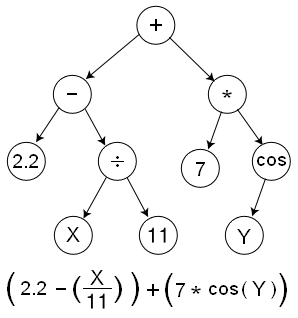
\includegraphics[scale=0.45]{Genetic_Program_Tree.png}
	\caption[A function represented as a tree structure.]{A function represented as a tree structure. Source: Wikipedia}
	\label{fig:Genetic_Program_Tree}
\end{figure}

\begin{figure}[htb]
	\centering
		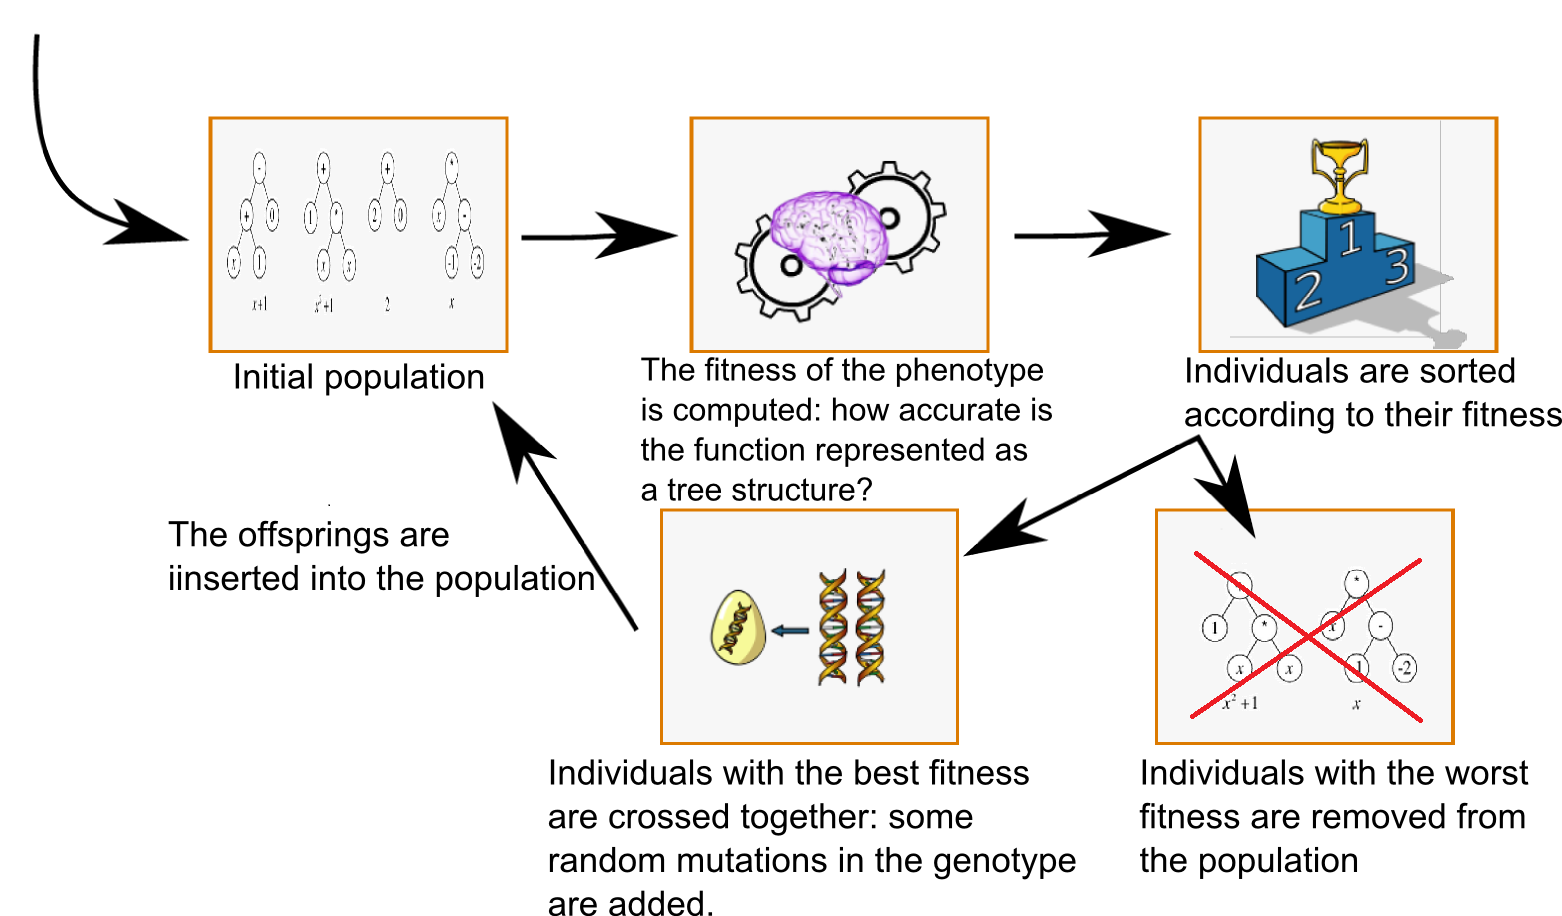
\includegraphics[width=0.8\textwidth]{genetic_programming_regression_synopsis.png}
	\caption[Functioning of an evolutionary algorithm]{Functioning of an evolutionary algorithm: from an initial population of solutions, they are ranked according to their fitness, the worst ones are eliminated and the best ones are used to produce new solutions.}
	\label{fig:algorithmes_evolutionnistes_synopsis}
\end{figure}

~~\\
Genetic programming is a perfect suit for symbolic regression. The term "symbolic regression" represents the process during which measured data are fitted by suitable mathematical formula like $x^2 + C$, $sin(x) + 1/e^x$,  etc. This process is quite well known amongst mathematician and is used when some data of unknown process are obtained. The domain of symbolic regression is of functional nature, i.e. it consists of a function set like ($sin()$, $cos()$, $gamma()$, $MyFunction()$,...) and so called terminal set ($t$, $x$, $p$, ...). From a mix of both sets is then synthesized the final program, which can have a complicated structure. We plan to use genetic programming for symbolic regression in order to unravel unknown relation between some given attributes of a relation.   


\subsubsection{Madlib Implementation}
TODO

DEAP

Appendix \ref{sec:app:implementation} gives details on the technical aspects of the implementation.

\subsection{Adaptive Boosting}
\subsubsection{Background}
Boosting is one of the most important developments in classification methodology. Boosting works by iteratively applying a classification algorithm to re-weighted versions of the training data and then taking a weighted majority vote of the sequence of classifiers thus produced. For many classification algorithms, this simple strategy results in dramatic improvements in performance. While boosting has evolved over the years, we focus on the most commonly used version of boosting known as Adaptive Boosting (AdaBoost) for binary classification developed by Freund and Schapire~\cite{boost96}.

Let us look at a concise description of AdaBoost in a two-class classification setting. We have training data $(x_1, y_1), \ldots, (x_n, y_n)$ with $x_i$ a vector valued feature and $y_i = -1\text{ or }1$. We define $F(x) = \sum_1^M{c_mf_m(x)}$ where each $f_m(x)$ is a classifier producing values $1\text{ or }-1$ and $c_m$ are constants; the corresponding prediction is $\text{sign}(F(x))$. The AdaBoost procedure trains the classifiers $f_m(x)$ on weighted versions of the training sample, giving higher weight to cases that are currently misclassified. This is done for a sequence of weighted samples, and then the final classifier is a linear combination of the classifiers from each stage. The pseudocode for AdaBoost is given in Figure~\ref{fig:adaproc}.

\begin{figure}[ht]
\centering
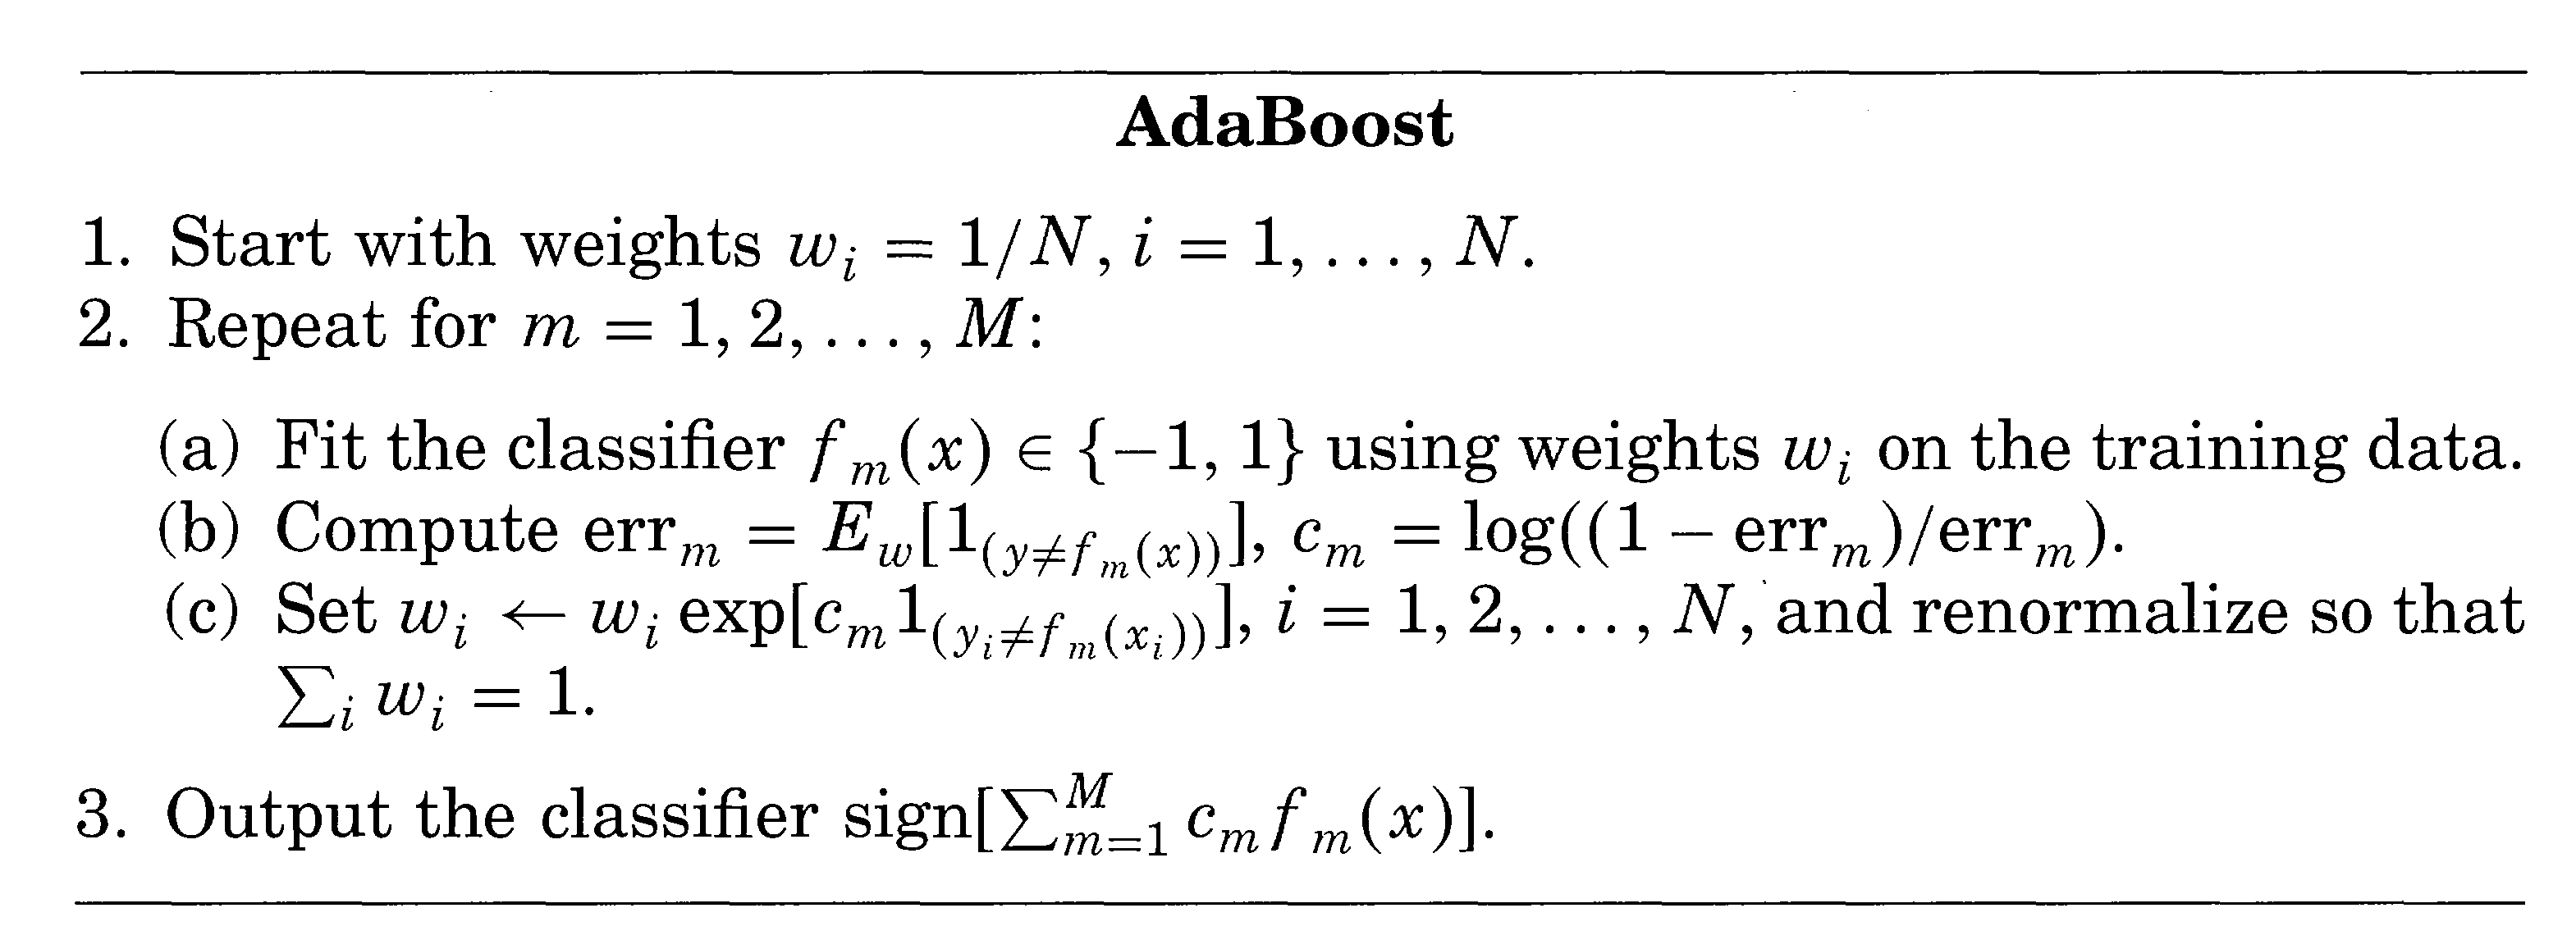
\includegraphics[width=0.8\textwidth]{ada.png}
\caption{AdaBoost algorithm. $E_w$ represents expectation over the training data with weights $w=(w_1,w_2,\ldots,w_N)$ and $I_{(S)}$ is the indicator of the set $S$~\cite{alr00}.}
\label{fig:adaproc}
\end{figure}

We used ``Stumps'' as weak learners. Stumps are single-split trees with only two terminal nodes. Stumps are simple to implement, typically have low variance and success of boosting depends on variance reduction~\cite{alr00}.


\subsubsection{Madlib Implementation}
 

\section{Benchmark}
\label{sec:bench}
In this section, we show the results of the benchmarks that we performed to assess the performance of our implementations in various settings. We also discuss the implications of the results that we found.
\subsection{Setup}
We ran the benchmark on PostgreSQL 9.1.9 and MADlib v0.3 on a single machine on a gigabit Ethernet cluster which runs Ubuntu 12.04 LTS and has 4GB RAM, a 10GB SATA HDD and a Core 2 Duo 2.4GHz CPU. 

To benchmark the performance of GP for Symbolic Regression we used a synthetic dataset containing 100,000 rows, 3 inputs and 1 output. The function we used to generate the data is $x_1*(x_2^2+x_3)$.

To benchmark the performance of AdaBoost, we used BUPA liver disorder dataset which contains blood test results of 345 male individuals. This dataset is available at \url{http://www.cs.huji.ac.il/~shais/datasets/ClassificationDatasets.html}. We also used a synthetic dataset which consisted of $240000\times11$ matrix where first 10 columns are real valued random numbers and the last column indicates the class.

Each run of our algorithms inside MADlib was cold start meaning that we cleared the caches and restarted the database service (PostgreSQL) for every run.


%\subsection{Results}
%Tables~\ref{tab:gp}, \ref{tab:adaBupa1}, \ref{tab:adaBupa2}, \ref{tab:adaSynth1} and \ref{tab:adaSynth2} in Appendix A summarize our benchmark results. Table~\ref{tab:gp} shows <Filled by Franck>. In Table~\ref{tab:adaBupa1}, we record the runtimes of row-by-row execution, batched execution and all-in-memory execution of AdaBoost inside MADlib. In Table~\ref{tab:adaBupa2}, we record the runtimes of the same algorithm when it reads data from a file or from PostgreSQL database outside MADlib or loads data into memory from Postgres residing inside MADlib. In all cases we varied the number of iterations parameter. Table~\ref{tab:adaSynth1} shows the runtimes and Table~\ref{tab:adaSynth2} shows the memory usage of row-by-row execution, batched execution and all-in-memory execution of AdaBoost when it is run on a synthetic dataset of varying size.    

%As we can see from the tables, the runtime of both of the algorithms increases as we increase the number of independent variables. Running the algorithms using MADlib takes more time than bypassing MADlib altogether when data can be fit into memory. Running the algorithms using MADlib is advantageous when the dataset cannot be fit into memory. Batched execution is more efficient in terms of run time than row by row execution in terms of run time. It is more efficient than reading the whole dataset into memory in terms of memory usage.

\subsection{Result analysis}
\subsubsection*{\itshape Effect of varying independent variables on runtime and memory usage.}

The first focus of our analysis was the effect of the parameters of the synbolic regression and of AdaBoost on the runtime and memory usage. Figure \ref{fig:gp-inside-vs-outside} shows that as expected when we increase the value of our parameters, it increases the runtime proportionally. By the same token, as expected increasing the size of the data set cause PostgreSQL to use a higher amount of memory.


\begin{figure}[ht]
\centering
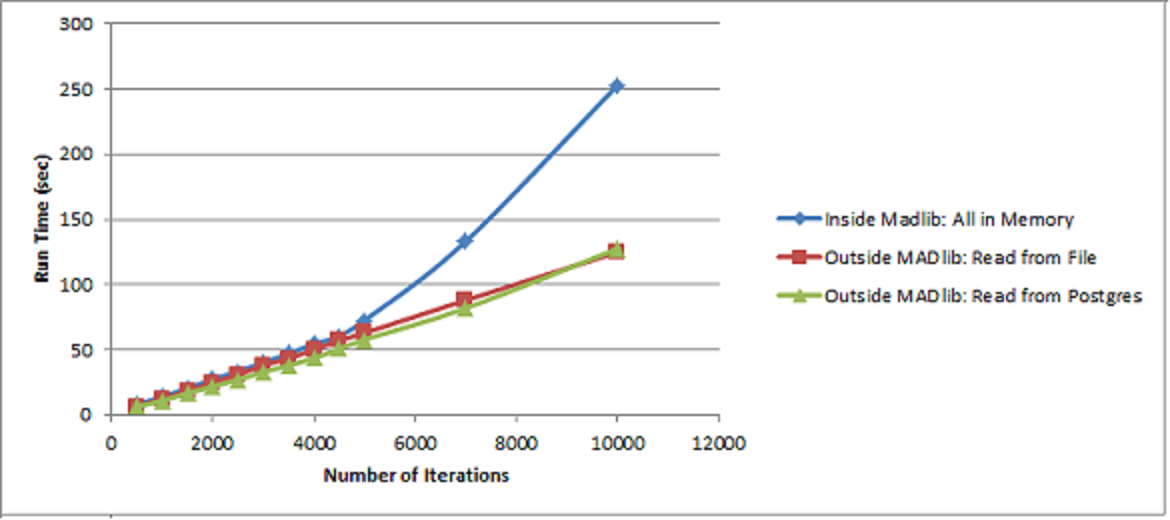
\includegraphics[height=180px]{ada1.png}
\caption{Runtimes of AdaBoost algorithm inside and outside MADlib.}
\label{fig:adainout}
\end{figure}


\begin{figure}[ht]
\centering
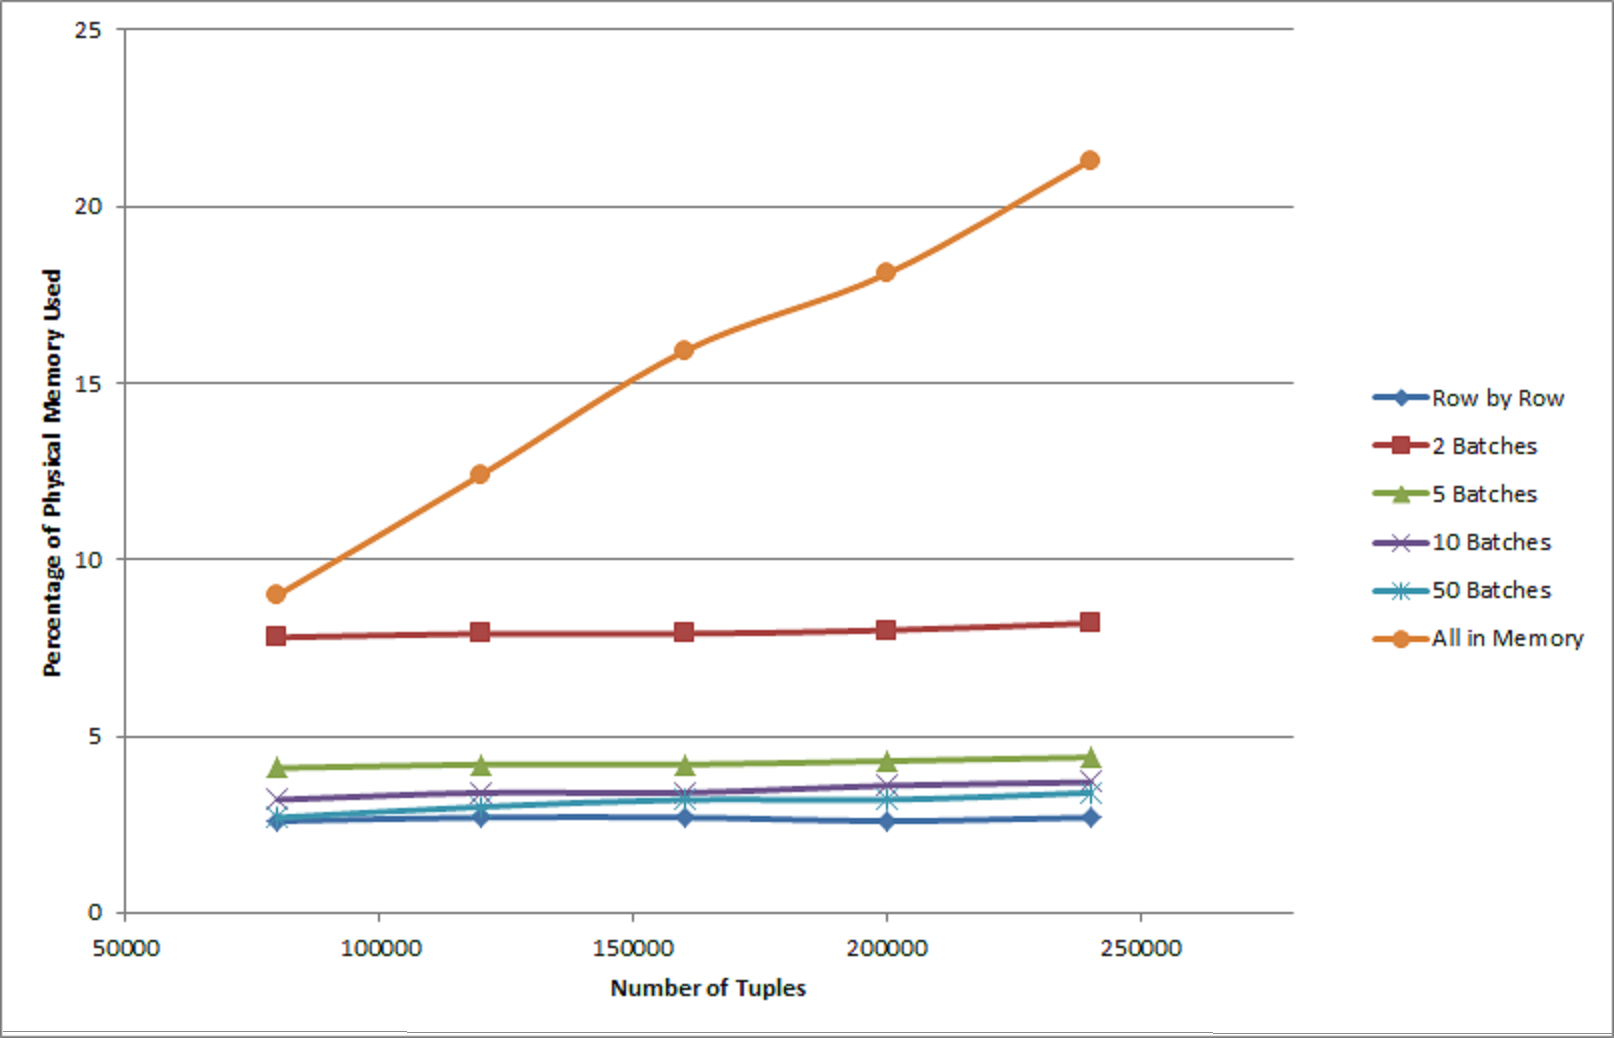
\includegraphics[height=180px]{ada4.png}
\caption{Memory usage by AdaBoost algorithm on synthetic dataset.}
\label{fig:adamem}
\end{figure}

\begin{figure}[ht]
\centering
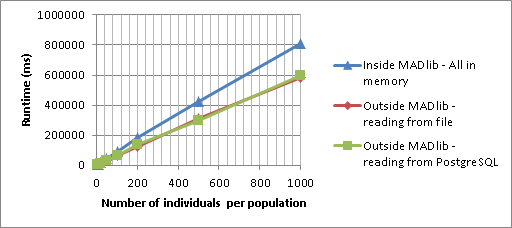
\includegraphics[height=180px]{gp-inside-vs-outside.png}
\caption{Runtimes of symbolic regression inside and outside MADlib.}
\label{fig:gp-inside-vs-outside}
\end{figure}

\subsubsection*{\itshape Performance inside and outside MADlib}
Figure \ref{fig:gp-inside-vs-outside} also compares the runtime between different execution environments: within MADlib, outside MADlib reading from a file and outside MADlib reading from the PostgreSQL database. The code used was strictly identical in older to ensure a fair comparison between execution environments. Also, all the data was loaded in memory at the beginning of the program.

~~\\
First of all, in the case of the dataset that we used to perform symbolic regression, which contains 100,000 rows and of size 2686 KB, on average reading from a file takes 230 ms whereas it takes 510 ms reading from the PostgreSQL database. TODO: Sumaiya, explain your difference.

~~\\
The most intriguing result is the runtime within MADlib, which is significantly slower than the runtime outside MADlib. This result cannot be explain by the fact that querying the database makes running within MADlib slower since running outside MADlib reading from the PostgreSQL doesn't have the issue, and the difference of runtime increases when the number of iterations increases, which means the reason isn't a fixed cost.

~~\\
To investigate this difference of runtime we bypassed MADlib and created PL/Python test case that narrows down the issue:

\begin{verbatim}
CREATE FUNCTION testcase (b integer)
  RETURNS float
AS $$
  import time
  start = time.time()
  a = 0
  for i in range(b):
    for ii in range(b):
      a = (((i+ii)%100)*149819874987)
  end = time.time()
  plpy.info("Time elapsed in Python: " + str((end - start)*1000) + ' ms')
  return a
$$ LANGUAGE plpythonu;
\end{verbatim}

We compared the latter code with the following identical Python code:
\begin{verbatim}
import time
import sys

def testcase (b):     
    a = 0
    for i in range(b):
        for ii in range(b):
            a = (((i+ii)%100)*149819874987) # keeping Python busy
    return a

def main():    
    numIterations = int(sys.argv[1])        
    start = time.time()
    print testcase(numIterations)
    end = time.time()
    print "Time elapsed in Python:"
    print str((end - start)*1000) + ' ms'        

if __name__ == "__main__":
    main()
\end{verbatim}

~~\\
On our benchmark server, calling the PostgreSQL PL/Python function using \textit{select * from testcase(20000);}, it takes on average 65 seconds, while when we call the usual Python script with 20000 as argument too it takes an average 48 seconds. The averages were computed running the queries and scripts 10 times. This result means that for some reason the CPython that is embedded in PostgreSQL 9.1 is slower than the Python 2.7.3 we use outside PostgreSQL.

~~\\
We tested with PostgreSQL 9.2 (with Ubuntu 12.10 this time), and we still notice a runtime difference on my server (although overall 10\% faster, probably due to some new version of CPython). We also tried using plpython3u, which implements PL/Python based on the Python 3 language variant. plpythonu that we used before is equivalent to plpython2u, which implements PL/Python based on the Python 2 language variant. Using plpython3u is far slower (88 seconds), but when running the Python script using python3 it is also slower (75 seconds), although still significantly faster than plpython3u.

~~\\
TODO: try on my VM and conclude


\subsubsection*{\itshape Performance of batched execution.}

So far our modules have loaded all the data in memory, then performed the computations on them. However, in some situation we might not have enough memory to store all the data. In older to circumvent this issue our modules allow to define the amount of memory the user wants to grant to the module. To do so, the user can choose the batch size, which corresponds to the number of rows the module can put in memory. At each iteration of the algorithm, we retrieve data in batches. Since we cannot store them in memory, it means we will have in total an important amount of queries to the database. The smaller the memory the user grants to the module, the higher the amount of queries to retrieved data at each iteration will be.

~~\\
Figure \ref{fig:gp-batch-histo} shows the effect of the batch size in the case of the symbolic regression. We fixed the parameters and only changed the batch size. As we can see, having a batch size of 10,000 rows or a batch size of 1,000 rows is a pretty good trade-off: for batch size = 10,000 rows, the runtime is 1.5  times bigger, and for batch size = 1,000 rows, the runtime a bit less than twice bigger. TODO: add reference to the table in the appendix. Since the memory used is proportional to the batch size, it makes using large batches look attractive. However, if we further decrease the batch size, we see that it starts having a very negative impact on the runtime.

~~\\
Figures \ref{fig:adabatch1} and \ref{fig:adabatch2} shows the impact of the batch size on the runtime when the number of iterations increases.

~~\\
Table~\ref{tab:adaSynth1} shows the runtimes and Table~\ref{tab:adaSynth2} shows the memory usage of row-by-row execution, batched execution and all-in-memory execution of AdaBoost when it is run on a synthetic dataset of varying size. 


\begin{figure}[ht]
\centering
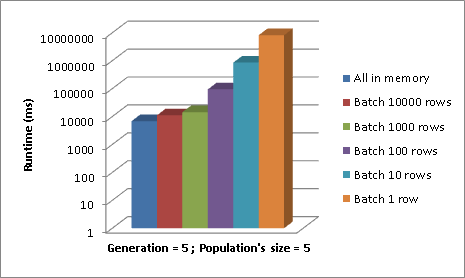
\includegraphics[height=180px]{gp-batch-histo.png}
\caption{Runtimes of row-by-row, batched and all-in-memory execution of symbolic regression. The dataset contains 100,000 rows. Having a batch size of 10,000 rows means that at each iteration we do $100,000/10,000 = 10$ queries on the database}
\label{fig:gp-batch-histo}
\end{figure}

\begin{figure}[ht]
\centering
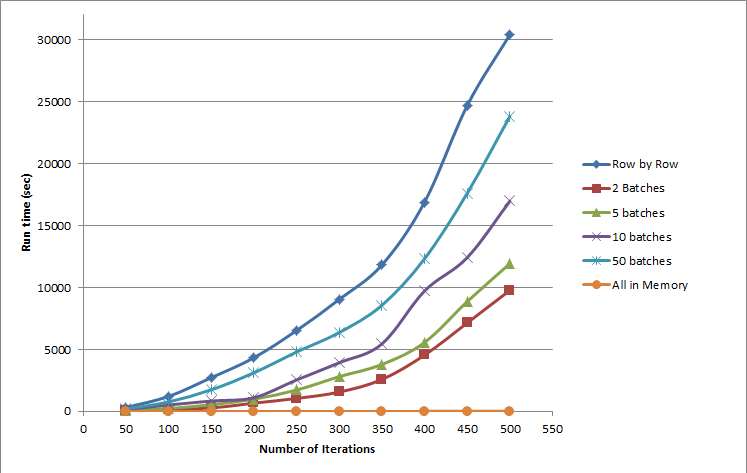
\includegraphics[height=180px]{ada2.png}
\caption{Runtimes of row-by-row, batched and all-in-memory execution of AdaBoost algorithm on BUPA liver disorder dataset.}
\label{fig:adabatch1}
\end{figure}

\begin{figure}[ht]
\centering
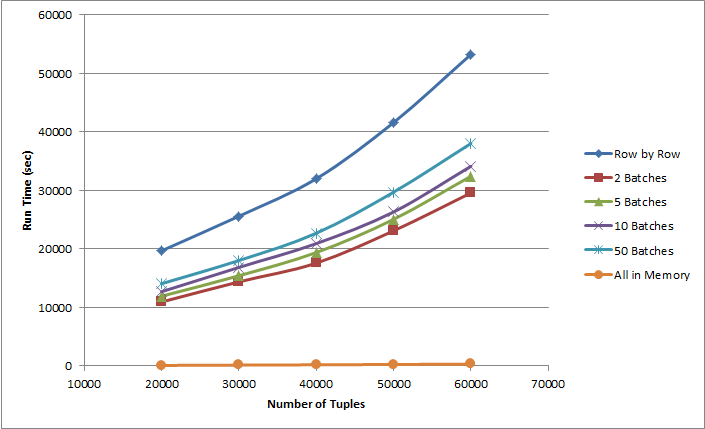
\includegraphics[height=180px]{ada3.png}
\caption{Runtimes of row-by-row, batched and all-in-memory execution of AdaBoost algorithm on synthetic dataset.}
\label{fig:adabatch2}
\end{figure}

 

\section{Conclusions}
\label{sec:con}


\bibliographystyle{plain}
\bibliography{report}
\pagebreak

\section*{Appendix A: Installing Madlib with PostgreSQL}


These instructions have been tested on Ubuntu 12.04 x64. It won't work with Ubuntu 12.04 x32 (MADlib does not have support for Ubuntu 32-bit). Also, MADlib doesn't work with GCC 4.7.*, so since Ubuntu 12.10 ships with GCC 4.7.2 it might be an issue.

~~\\
\# install postgres packages \\
sudo apt-get -y install postgresql-9.1 libpq-dev postgresql-server-dev-9.1 postgresql-plpython-9.1

\# Download madlib from http://madlib.net and copy tar file to server \\
wget https://github.com/madlib/madlib/zipball/v0.5.0
unzip v0.5.0
cd madlib-madlib-5fabd88 

\# Build Madlib \\
sudo apt-get -y install cmake
sudo apt-get -y install m4 gcc-4.6 g++-4.6 g++
./configure
cd build/
make
make doc
make install

\# To connect to the database: \\
sudo su - postgres
psql

\# To add a password to a role: (note: might be more convenient to use a 1-letter password when coding for MADlib as we'll keep having to enter the password each time we reinstall it) \\
postgres=\# alter role postgres with password 'postgres';

\# To register Madlib with the postgres database \\
/usr/local/madlib/bin/madpack -p postgres -c \$USER@\$HOST/postgres install

\# To test your installation you can run the install check procedure: \\
/usr/local/madlib/bin/madpack -p postgres -c \$USER@\$HOST/\$DATABASE install-check


\section*{Appendix B: Installing a module in Madlib}


\section*{Appendix C: Sample run of GP}


\section*{Appendix D: Sample run of AdaBoost} 

\end{document}
